
\section {Introduction}

\begin{figure}
\centering
     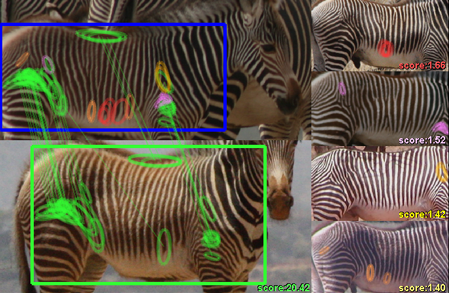
\includegraphics[width=\linewidth] {figures/FinalImages/FoalSystemCropped.png}
\caption{\footnotesize{An example of HotSpotter. The ROI is placed on a
  query animal --- in this case a foal --- and a ranked list of
  matching animal images from the database is returned.  Here, the correct
  match, an image of the same animal as an older juvenile, is the best match
  (top right).  The green ellipses show the matching regions, or ``hot
  spots'', between the two images.  Images along the bottom of the
  figure show significantly lower matching scores for different animals.}}
\label{fig:onevsone}
\end{figure}


\textbf{Motivation:}
Conducting research on animal populations
requires reliable information on the position and movement of individual
animals.  Traditionally, this information has been obtained by
attaching tags and transmitters to captured animals.  These methods
do not scale well to large populations, are expensive, physically invasive, and require proximity to unwilling
subjects \cite{wsb94ElbinMicrochipIden, acmss04ZhangZebraNet}.

The widespread availability of inexpensive, good-quality digital
cameras offers the promise of an alternative approach.  Images of
animals may be taken by anyone who has a camera --- scientists and
their assistants, ecotourists, and even ordinary citizens ---
producing the potential for enormous flood of image data.
Moreover, recent cameras include both a clock and a GPS unit, allowing
each image to also record location and time.

Fundamentally, exploiting the wealth of photographic data for animal
population analysis depends on locating and recognizing the animals in
each image.  The recognition step requires comparing each animal image
to a database of pictures of animals that have already been
identified, and then either adding to the record of a
previously known animal or creating an additional record for a new
individual.  Even for small populations of 100 animals,
doing this comparison manually is tedious and error prone.  It does
not scale at all to large populations.
Clearly, computer-based methods for automatic animal identification %Assisted identification, not automatic?
are needed.

This need has spawned research on recognition of
animals ranging from penguins to zebras to whale sharks \cite{ipc10SherleyCVPenguin, jae05HolmbergAstroWhaleShark}.  Some methods
are species specific \cite{si04BradfieldFrogPhoto, aje09ShorrocksNeckNet, icmr11LahiriStripeSpotter},
while others have strived for generality \cite{fiz07SpeedSpotMatch, 11BoldgerWILDID}.
In particular, the Wild-ID algorithm of Bolger \etal~\cite{11BoldgerWILDID} employs
keypoint matching techniques
from computer vision literature \cite{ijcv04LoweSIFT} to
determine if two images show the same
animal. In our paper, we build on more recent methods from the computer %animal instance, individual ...
vision literature to take an important step beyond this, creating both
an improved method for matching two images
and a fast method for matching against the entire database
without sequential image-to-image matching. %took out even more images. There could be more animals than images

\textbf{Problem Statement:} Our computational task is as follows.  We
are given a database of labeled images, where each label identifies
(names) the individual animal in the image. The same animal may
appear in more than one database image. We keep multiple images to
accommodate viewpoint differences and appearance changes.  Given
a novel query image, $I_Q$, and a
manually-specified rectangular region of interest (ROI) locating the
animal in the image, our goal is to
assign a label to the animal in the ROI or to decide that the animal has
not been seen before.  More practically, the goal is modified
slightly: to provide a set of potential animal labels from the
database ranked by a similarity score.
A high score should indicate a highly probable match,
while low scores should indicate improbable matches.
Figure~\ref{fig:onevsone} shows an example.

Three comments about this problem are appropriate.  First, user
interaction is required only to select the animal ROI in the query image
and to verify the labeling results.  Ongoing work will replace both of
these with more automated methods, but some user interaction will
always be necessary, both for the hardest cases and to build user
confidence in the system.
Second, for the current work, we assume the collection protocol has produced images all of one flank of the animals, avoiding the ambiguity associated with seeing two different sides of the same animal.
Third, for the experiments in this paper,
the database of animal images and labels is
static. In practice, however, the database will be dynamic.  We bias
our selection of techniques in light of this, and the system
described here is already in use with a changing image set.
However, fully addressing the issues of a efficiently searchable, large-scale, and dynamic
database of animal images is beyond the scope of this paper.

\textbf{Algorithm Overview:} We present two algorithms to solve the
animal identification problem.  A high-level summary of both is:
(a) for every image, the algorithms locate keypoints and extract associated descriptors (128-dimensional
vectors), and (b) they then determine image matches based on the comparison of these descriptors.

  The first algorithm is similar to Wild-ID
\cite{11BoldgerWILDID} in that it matches the query image
against each database image separately, sorting the database images by the
resulting similarity score in order to generate the final ranked
results.  This is our \emph{one-vs-one} matching algorithm, and
it contains several minor improvements over Wild-ID that result in a more robust
algorithm.

Our second algorithm, which we refer to as the \emph{one-vs-many}
algorithm, matches each descriptor from the query image against
\textbf{all} descriptors from the database image using a fast,
approximate nearest neighbor search data structure.  It generates scores
for each database image based on these matches, and then aggregates
the scores to produce the final, overall similarity score for each
individual (each label).  In addition to introducing fast matching to the animal
identification problem, our most important contribution here is a new
mechanism for scoring descriptor matches based on the Local Naive Bayes Nearest %matching->match
Neighbor methods \cite{cvpr11McCannLNBNN}.

\textbf{Dataset:} We test our algorithms, which are currently in use in the
field in Kenya, on five different species of animals: giraffes,
jaguars, lionfish, plains zebras and Grevy's zebras.  Our most
extensive databases are for the zebras, so these are the focus of the
experiments in this paper.




